\section{Реализация набора динамических библиотек}

%---------------------------------------------------------
%Highlighting text
\begin{frame}
\frametitle{Проектные решения для динамических библиотек}

В предыдущих версиях Unix Taskbook были оставлены интерфейсы, которые облегчают расширение на большее количество различных групп задач.



\begin{figure}[htbp]%
    \centering
    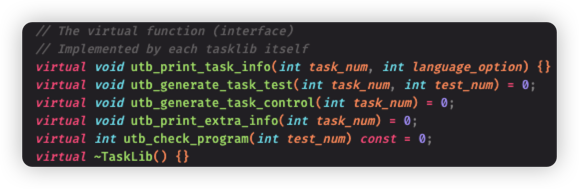
\includegraphics[width=0.8\linewidth]{images/tasklib.jpg}%子图文件名
    \caption{Tasklib.}%总标题
    \label{tasklib}%总标签
\end{figure} 

Эти интерфейсы предоставляются классом TaskLib, и классы, которые мы создаем сами, будут работать нормально, если они реализуют эти интерфейсы.

\end{frame}
%---------------------------------------------------------


%---------------------------------------------------------
%Two columns
\begin{frame}
\frametitle{MPI1Proc}
\begin{example}
MPI1Proc является одной из многих групп задач по параллельному программированию. Соответствующий класс динамической библиотеки - utbMPI1Proc.
\end{example}
\begin{figure}[htbp]%
    \centering
    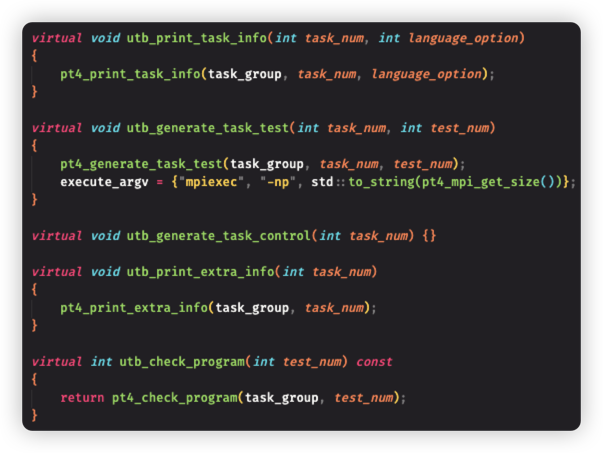
\includegraphics[width=0.5\linewidth]{images/1proc.jpg}%子图文件名
    \caption{MPI1Proc.}%总标题
    \label{proc}%总标签
\end{figure} 

\end{frame}
%---------------------------------------------------------

%---------------------------------------------------------

\begin{frame}{Вспомогательные файлы pt4utilities}

\begin{itemize}
    \item Поскольку наша задача состоит в адаптировать группы заданий, реализованные для Programming Taskbook \cite{ref2}, без переписывания связанного с ними программного кода.Поэтому нам необходимо передать управление этими группами задач нашей динамической библиотеке.Таким образом, была разработана программа pt4utilities.
    \item pt4utilities - это набор инструментов, который загружает базовые динамические библиотеки (Динамическая библиотека, содержащая эти группы задач , реализованные на языке Pascal), а затем получает контроль над исходной группой задач. Затем наша динамическая библиотека может управлять генерацией данных задачи, проверкой результатов задачи и т.д. через интерфейс, предоставляемый pt4utilities.
\end{itemize}

\end{frame}

%---------------------------------------------------------


%---------------------------------------------------------
%Two columns
\begin{frame}
\frametitle{pt4utilities}

\begin{figure}[htbp]%
    \centering
    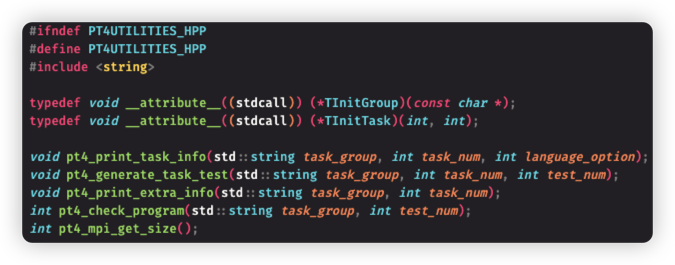
\includegraphics[width=0.9\linewidth]{images/pt4.jpg}%子图文件名
    \caption{pt4utilities.}%总标题
    \label{pt4}%总标签
\end{figure} 

\end{frame}
%---------------------------------------------------------

%---------------------------------------------------------
%Highlighting text
\begin{frame}
\frametitle{Модули обработки данных udata и uprint}

Для корректного отображения данных в терминале мы также разработали модуль, предназначенный для обработки данных, который имеет следующие функции:

\begin{itemize}
    \item Загрузка файлов данных;
    \item Проверка данных;
    \item Форматирование данных, чтобы сделать интерфейс более привлекательным.
\end{itemize}

\end{frame}
%---------------------------------------------------------